\section{Contribution}
\counterwithin{equation}{section}
The "Contribution" section of the thesis highlights the developed new method called \textbf{DannFixbi}, which combines the Fixbi approach and the backpropagation approach. In an attempt to implement the state-of-the-art method, extensive research has been conducted, and existing approaches have been implemented. The decision to combine these two approaches was based on their respective strengths and the potential for mutually beneficial interaction between them. By incorporating the Fixbi technique, which addresses domain shift, and leveraging the benefits of backpropagation, \textbf{DannFixbi} aims to enhance the performance and robustness of domain adaptation in the field of images. The development of \textbf{DannFixbi} represents an original contribution to the field. \\

This new method consists of two neural networks, which are trained using a modified version of the Fixbi approach. To enhance the performance of this method, two domain classifiers are added to each of these two networks. Two different approaches have been explored for incorporating these domain classifiers.\\

The first approach involves adding a domain classifier to each neural network (see Figure \ref{fig:dannfixmix}). During training, images obtained by mixing from the source and target domains with predefined mixup ratios are fed into these classifiers. 

\begin{figure}[H]
    \centering
    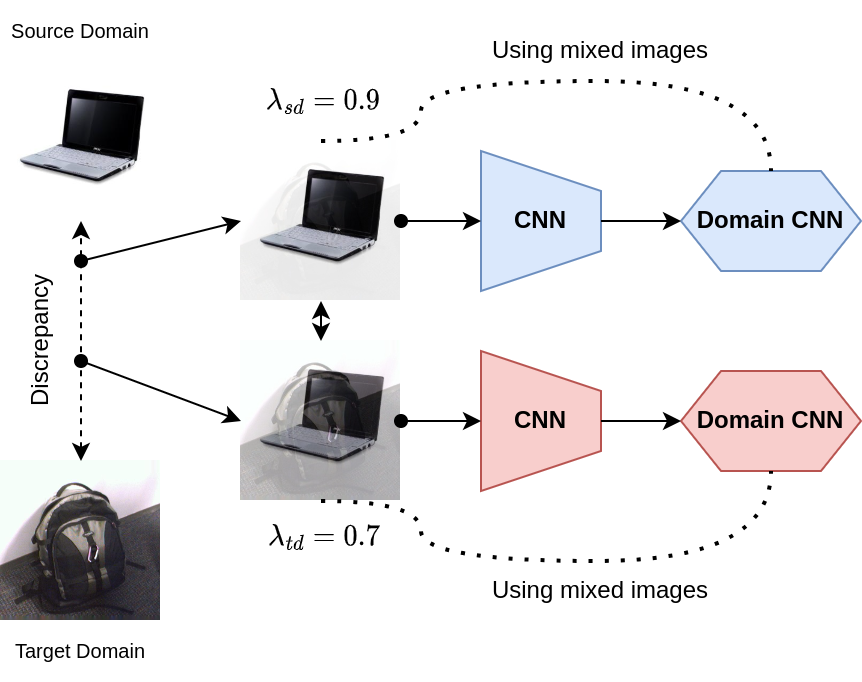
\includegraphics[width=0.55\textwidth]{Figures/Results/df_mix.png}
    \caption{\textbf{DannFixbi} architecture of the first approach.}
    \label{fig:dannfixmix}
\end{figure}

For mixed images, the following loss functions is used:

\begin{equation}
    L_{dom} = \alpha L_{ds}(\hat{X}, Y_{s}) + (1 - \alpha) L_{dt}(\hat{X}, Y_{t}) ,
\end{equation}


where $\hat{X}$ is mixed images, $Y_{s}$ is source domain labels, $Y_{t}$ is target domain labels and $\alpha \in \{\lambda_{sd}, \lambda_{td}\}$. $L_{ds}$ and $L_{dt}$ presents cross entropy loss for source and target domains, respectively.\\


The second approach is to use a domain classifier for each net with images from the source and target domains without any mixing, similar to the backpropagation method (see Figure \ref{fig:dannfixsep}).\\

\begin{figure}[H]
    \centering
    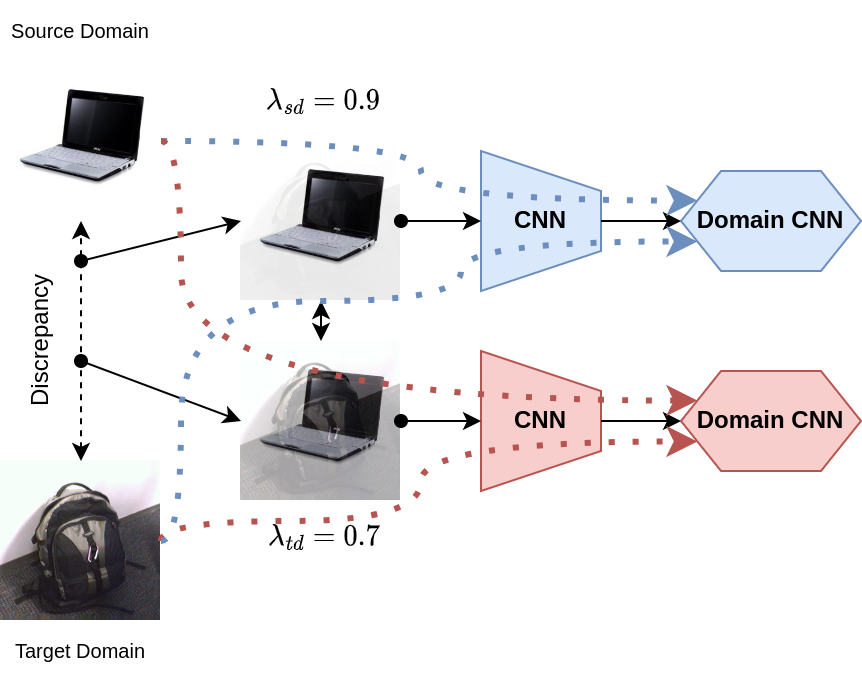
\includegraphics[width=0.55\textwidth]{Figures/Results/df_sep.png}
    \caption{\textbf{DannFixbi} architecture of the second approach.}
    \label{fig:dannfixsep}
\end{figure}

The second approach utilizes the following loss function for domain classification:

\begin{equation}
L_{dom} = L_{d}(X_{st}, Y_{st}) ,
\end{equation}

where $X_{st}$,  $Y_{st}$ denotes source and target images and domain labels, respectively, and $L_{d}$ is a cross entropy loss. \\

The total loss for the new method is calculated as the sum of the loss from the Fixbi method and the domain loss described earlier:

\begin{equation}
L_{total} = \beta L_{fixbi} + \gamma L_{dom}
\end{equation}

Here, $\beta$ and $\gamma$ represent the weights assigned to the Fixbi loss and the domain loss, respectively. The values of these weights determine the relative importance of each component in the overall loss calculation. Further, unless otherwise stated, the values of alpha and beta are assumed to be equal to 1. The Fixbi loss, denoted as $L_{fixbi}$, is composed of several summands described in the  equations \ref{eq:fixbi1} -- \ref{eq:fixbi4}: 

\begin{equation}
L_{fixbi} = L_{fm} + L_{sp} + \mathds{1}\{e > k\} \left(L_{bim} + L_{cr}\right)
\end{equation}
where $e$ denotes a current epoch, and $k$ is  warm-up epochs. To establish independent characteristics for the two networks, it is introduced a warm-up period of $k$ epochs. During this phase, each network is trained separately using the fixed ratio-based mixup and self-penalization techniques. Once an enough amount of training has been completed, bidirectional matching loss is added, which helps networks train collaboratively, exchanging knowledge and benefiting from each other's insights. \\

The new method, referred to as \textbf{DannFixbi}, demonstrates improved performance and robustness in unsupervised domain adaptation for image analysis. This contribution represents a unique approach to UDA, offering valuable insights and potential for future developments in this field. All the results obtained are presented in the "Experiments" section.
%using the second approach (unless otherwise stated)

\newpage
\counterwithin{equation}{subsection}
\section{Experimental Setup} \label{section: copy me}
%\lipsum[1-8]

In this part, we start with description of different datasets that are commonly used in transfer learning. Then, we will continue with implementation details and experiments that have been conducted. Code is available at \href{https://github.com/Jetwev/domain-adaptation}{https://github.com/Jetwev/domain-adaptation}.

\subsection{Datasets}

The most popular datasets are \textbf{Office-31}, \textbf{ImageCLEF-DA}, \textbf{Office-Home}, \textbf{DomainNet} and \textbf{VisDA-2017}. Detailed discussion of each of them is given below:

\begin{itemize}
    \item \textbf{Office-31} \cite{saenko2010adapting} consists of 4,110 images categorized into 31 classes, which are distributed across three separate domains: Amazon (A), Webcam (W), and Dslr (D).
    \item \textbf{ImageCLEF-DA}, utilized in \cite{long2017deep}, includes three distinct domains: Caltech-256 (C), ImageNet ILSVRC 2012 (I), and Pascal VOC 2012 (P). There are 600 images in each domain and 50 images for each category.
    \item \textbf{Office-Home} \cite{venkateswara2017deep}, includes four absolutely different domains: Artistic images (Ar), Clip Art (Cl), Product images (Pr) and Real-World images (Rw). This dataset contains 15~500 images in 65 object classes, which makes it more complex than Office-31.
    \item \textbf{VisDA-2017} \cite{peng2017visda} consists of 12 classes shared between two very different domains: Synthetic and Real. It contains synthetic images (training set) and real-world images (test set). The dataset was designed to have a large domain gap, which makes it a challenging benchmark for domain adaptation methods.
    \item \textbf{DomainNet} \cite{peng2019moment} is a large-scale visual recognition dataset designed to evaluate domain adaptation algorithms, which consists of almost 600 thousand images and includes 345 classes.
\end{itemize}

\newpage

\subsection{Implementation details}

At the beginning, it was necessary to start with some approaches to check their performance and have a possibility to compare results. Four different methods described in the papers have been chosen for the study:

\begin{itemize}
    \item \textbf{Source only} is a method where a model is trained solely on the source domain data without any adaptation to the target domain.
    \item \textbf{Domain-Adversarial Neural Network (Dann)} is domain adaptation technique that aims to learn a domain-invariant feature representation by aligning the feature distributions of the source and target domains. The architecture of Dann consists of three components: a feature extractor network, a label predictor network, and a domain classifier network, and is described in more details in section 2.1.
    \item \textbf{Moving Semantic Transfer Network (Mstn)} The key idea behind Mstn is to add semantic transfer loss to the Dann approach. In the section 2.2, it is proposed to use average centroid alignment for aligning the feature distributions of the source and target domains. The architecture is the same as in the Dann method. 
    \item  \textbf{Fixbi} is the approach described in details in the section 2.3. The main idea is to train two neural networks, allowing models to learn from each other or on their own results. For this purpose, the authors add bidirectional matching and self-penalization losses.
\end{itemize}

\textbf{CNN architectures.} For all approaches, pretrained Resnet50 \cite{he2016deep} is utilized as the backbone network. The weights for the neural network can be downloaded from this \href{https://download.pytorch.org/models/resnet50-19c8e357.pth}{link}. Resnet50 has been pretrained on large image datasets such as ImageNet, which means that the network has already learned to recognize a wide range of features in images. Resnet50 is a convolutional neural network architecture consisting of 50 layers. This is a variant of the Resnet family of neural networks, which are designed to solve the vanishing gradient problem in deep neural networks. Resnet networks achieve this by using short connections between layers, which allow gradients to move more easily during backpropagation. Resnet50 is a widely used architecture in many articles, which makes it a good choice for research.\\ 

Resnet50 is used as a \textit{Feature extractor} in all considering methods. \textit{Label predictor} is a simple network that consists of two fully connected layers ($2048 \rightarrow 256 \rightarrow \textit{number of classes}$). \textit{Domain classifier} architecture represents several fully connected layers with a ReLU activation function and dropouts between each two fully connected layers. Using dropouts can reduce the sensitivity of the model to specific features in the input data and encourage the model to learn more generalizable features. This can lead to better performance on new, unseen data and can prevent overfitting. \\

%($2048 \rightarrow 1024 \rightarrow 256 \rightarrow 32 \rightarrow \textit{number of domain}=2$)

\textbf{Learning rate schedulers.} Learning rate is an important hyperparameter that determines the step size at which the optimizer updates the model's parameters during training. There are many of them and it can be challenging to find the optimal learning rate, as setting it too high can cause the model to diverge, while setting it too low can slow down the learning process. Thus, in this study it is utilized two different learning rate schedulers: \textit{CustomLRScheduler} and \textit{CosineAnnealingLR}. The implementation of the first one follows the rules that are described in \cite{ganin2015unsupervised} 

\begin{equation}
    \eta_p = \dfrac{\eta_0}{(1 + \alpha \cdot p)^\beta},
\end{equation}

where $p$ linearly increases from $0$ to $1$, and the values $\eta_0$, $\alpha$, and $\beta$ are set to $0.01$, $10$, and $0.75$, respectively. The second one, \textit{CosineAnnealingLR} is a popular learning rate scheduler utilized in deep learning. It systematically reduces the learning rate over multiple epochs in a cyclical manner. Initially, the learning rate starts at its maximum value and then gradually decreases until it reaches the minimum value. Upon reaching the minimum value, the cycle restarts, and the learning rate returns to its maximum value. This process continues until the end of the training, which is usually determined by the total number of epochs or a predefined stop criterion. By starting with a higher learning rate and gradually decreasing it, the model can avoid getting stuck in local minima and converge to a better global minimum. The formula for the \textit{CosineAnnealingLR} scheduler is:

\begin{equation}
\eta_t = \eta_{min} + \dfrac{1}{2}(\eta_{max} - \eta_{min}) \left(1 + \cos \left( \dfrac{T_{cur}}{T_{max}} \pi \right)\right),
\end{equation}

where $\eta_{max}$ is your initial learning rate, $\eta_{min}$ -- minimum learning rate value, $T_{cur}$ is the number of epochs since the last start, $T_{max}$ -- the total number of epochs. More detailed information about \textit{CosineAnnealingLR} can be found \href{https://pytorch.org/docs/stable/generated/torch.optim.lr_scheduler.CosineAnnealingLR.html}{here}.\\

\textbf{Optimizers.} This study uses two popular optimization algorithms - stochastic gradient descent (\textit{SGD}) and adaptive moment estimation (\textit{Adam}). Both algorithms are commonly employed in deep learning to optimize the parameters of a neural network and improve its performance. \\

\textit{SGD} is a simple and popular optimization algorithm that updates the weights of a model in the direction of the negative gradient of the loss function. One limitation of \textit{SGD} is that it can get stuck in local minima and struggle with noisy or sparse gradients. To tackle this problem, several modifications can be used. In PyTorch, the \textit{SGD} optimizer has several hyperparameters that can be tuned to improve its performance. The following parameters (except learning rate) are considered in this study: 

\begin{itemize}
    \item \textbf{Momentum} is a hyperparameter that determines how much past gradients affect the current gradient update. It helps to minimize the impact of the noise and fluctuations in the gradient updates. However, setting the momentum too high can also lead to slower convergence.
    
    \item  \textbf{Weight decay} is a form of L2 regularization that adds a penalty term to the loss function during training. This penalty term is proportional to the square of the weights in the network, which encourages the model to use smaller weights and reduce overfitting.

    \item \textbf{Nesterov momentum} is a variant of momentum that takes into account the momentum term in the calculation of the gradient. This can help to reduce oscillations and improve convergence rates, especially in high-dimensional optimization problems.
\end{itemize}

\textit{Adam} is another optimization algorithm that is commonly used in deep learning. It is an extension of SGD. The key idea behind Adam is to maintain a separate adaptive learning rate for each parameter in the network, based on estimates of the first and second moments of the gradients. This makes Adam more effective than SGD for optimization problems with noisy or sparse gradients. However, it may not always be the best choice for every task and model architecture, so it's important to experiment with different optimization algorithms and settings to find the best approach for your specific problem. \textit{Adam} is considered in this study with default parameters, more information about the implementation and usage can be found at this \href{https://pytorch.org/docs/stable/generated/torch.optim.Adam.html}{link}.\\

\textbf{Pytorch Lightning.} PyTorch Lightning is a lightweight PyTorch wrapper that allows users to focus on the high-level design of their experiments and models, instead of dealing with the low-level implementation details. It provides a structured way to organize PyTorch code, making it easier to read and maintain.\\

PyTorch Lightning offers a range of benefits that make it a good choice for deep learning researches. Firstly, it offers a modular design that makes it easy to organize code. It gives you a convenient and user-friendly interface to manage and run experiments. Moreover, all these benefits can help to improve your productivity. Secondly, PyTorch Lightning makes it easier to scale models to multiple GPUs, which can significantly reduce training times for large models. Finally, it is flexible and can be easily integrated with other PyTorch libraries. Overall, PyTorch Lightning is an excellent choice for researchers who want to focus on the research aspect of deep learning and leave the engineering components to the library. More information can be found on the official \href{https://www.pytorchlightning.ai/index.html}{website}.\\

\textbf{Weights and Biases.} Weights and Biases (WandB) is a platform  that provides a suite of tools to help developers and data scientists track and visualize their machine learning experiments. WandB makes it easy to log, keep track of your progress and compare different experiments, visualize model performance, and collaborate with team members. One of the main advantages of WandB is its integration with popular machine learning frameworks such as TensorFlow, PyTorch, and Keras. This means that you can easily log and track your model's hyperparameters and performance metrics during training and evaluation. Moreover, WandB is a cloud-based platform, which means that users can access their experiments and data from anywhere with an internet connection and also share them with colleagues and co-workers. For more detailed information, it is recommended to visit the official \href{https://wandb.ai/site}{website}.\\ 

\textbf{Batch size.} Different domains in your dataset can contain different number of images that makes your training process more complicated. To tackle this problem, it is proposed two approaches. \\

The first one is to find the ratio of the smaller dataset size to the larger one and concatenate the smaller dataset multiple times to ensure that the number of batches is aligned during the training loop. However, it is important to emphasize that with this approach, overfitting can occur if the appropriate number of epochs is not established. This is because the smaller dataset will be fed into the model more times than the larger one (depends on the ratio).\\

The second approach involves varying the number of images taken per batch for each domain. Applying this approach, it becomes possible to avoid concatenating the smaller dataset multiple times, which effectively reduces the amount of memory consumed. It is crucial to carefully consider the number of images per batch, as choosing a value that is either too high or too low can have negative consequences.\\

\textbf{Augmentation techniques.} Augmentation techniques for images are used to create variations and increase the size of the training dataset by applying a series of transformations. These techniques are widely employed in computer vision tasks, including image classification, object detection, semantic segmentation, etc. Augmentation helps increase the diversity of the dataset, leading to improved model generalization and robustness. PyTorch provides a variety of image augmentation techniques. The following transformations are used in this research:

\begin{itemize}
    \item \textbf{Normalize} -- normalizes the image by subtracting the mean value and dividing by the standard deviation. 
    \item \textbf{Resize} is a function that allows you to resize an image to a specific size.
    \item \textbf{RandomCrop} is a function that randomly crops a portion of the image.
    \item \textbf{CenterCrop} is a transformation that allows you to perform a center crop on an image.
    \item \textbf{RandomHorizontalFlip} -- randomly flips the image horizontally with a specified probability.
    \item \textbf{RandomVerticalFlip} - randomly flips the image vertically with a specified probability.
    \item \textbf{RandomRotation} is a function that randomly rotates the image by a given angle.
    \item \textbf{ColorJitter} is a transformation that allows you to adjust the brightness, contrast, saturation, and hue of the image.
    \item \textbf{ToTensor} is a specific function in PyTorch that is used to convert an image into a tensor.
\end{itemize}

These augmentation techniques can be applied individually or combined sequentially using the \textit{transforms.Compose} function. More detailed information about transformations and their usage can be found \href{https://pytorch.org/vision/stable/transforms.html}{here}. It's important to emphasize that the choice and combination of augmentation techniques depend on the specific task and dataset characteristics, and careful selection of them are crucial to achieve optimal results.\\

\textbf{OmegaConf.} OmegaConf is a library for Python that provides a convenient and flexible way to manage complex configurations in machine learning projects. It is designed to provides a number of features that can help to simplify the configuration process. Here are some reasons why OmegaConf can be a good choice:

\begin{itemize}
    \item It is easy to use and allows developers to define nested configurations and easily access and modify configuration values.
    \item OmegaConf supports a wide range of configuration formats, including YAML and JSON. This makes it flexible and easy to integrate in your project.
    \item It supports type checking, which can help to catch configuration errors and improve code quality.
\end{itemize}
 
To sum up, OmegaConf can be a good choice for Python developers who work on large and complex projects and want a flexible and powerful configuration system for their applications. Additional details can be found \href{https://omegaconf.readthedocs.io/en/2.3_branch/}{here}.

\newpage

\subsection{Experiments}

The dataset \textbf{Office-31} is used to test the approaches. This dataset consists of three domains: Amazon (A) - 2817 images, Dslr (D) - 498 images and Webcam (W) - 795 images (see Figure \ref{fig:office}). 

\begin{figure}[H]
    \centering
    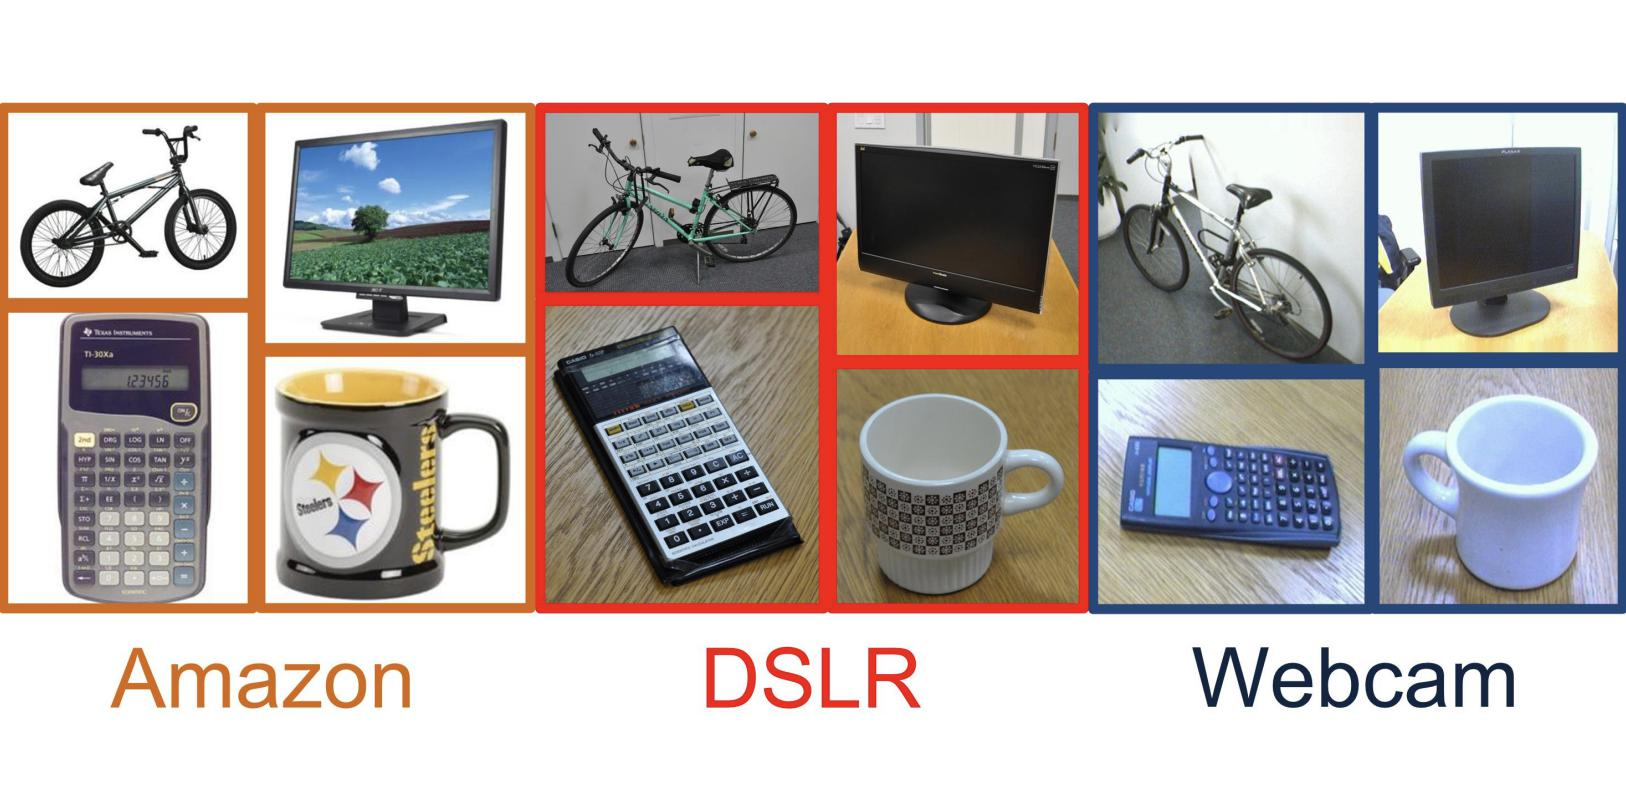
\includegraphics[width=0.9\textwidth]{Figures/Results/office-31.jpg}
    \caption{Different domains in dataset \textbf{Office-31}.}
    \label{fig:office}
\end{figure}

The Table \ref{tab:features} below highlights various key features of the dataset, including the number of classes, image resolution, task and evaluation metric.

\begin{table}[h]
\centering
\caption{General information about the Office-31 dataset}
\label{tab:features}
\begin{tabular}{|l|l|}
\hline
\textbf{Feature}  & \textbf{Description}                     \\ \hline
Dataset Name      & Office-31                                \\ \hline
Purpose           & Domain adaptation and object recognition \\ \hline
Number of Classes & 31                                       \\ \hline
Domains           & Amazon, Webcam, DSLR                     \\ \hline
Image Resolution  & Varies across domains and images         \\ \hline
Image Format      & JPG                                     \\ \hline
Task              & Multi-class classification               \\ \hline
Evaluation Metric & Classification accuracy                  \\ \hline
\end{tabular}
\end{table}

The existence of dissimilar image quantities ensures us in the importance of utilizing one of the approaches discussed in the previous section in order to avoid any information loss. In the first approach, where the smaller domain is concatenated, a batch size of 32 or 64 is utilized for all experiments. The second approach takes into account the size of each domain, and as a result, the batch sizes are utilized in the experiments according to the Table \ref{tab:batchsizes}:

\begin{table}[H]
\centering
\caption{The table of batch sizes is organized such that the numerical values in the first column correspond to the first letter, the second one to the second letter.}
\label{tab:batchsizes}
\begin{tabular}{|p{1.5cm}|p{1.5cm}|p{1.5cm}|}
\hline
   & \multicolumn{2}{l|}{Batch size} \\ \hline
\textit{AD} & 45   & 8   \\ \hline
\textit{AW} & 45   & 13  \\ \hline
\textit{DA} & 8    & 45  \\ \hline
\textit{DW} & 20   & 32  \\ \hline
\textit{WA} & 13   & 45  \\ \hline
\textit{WD} & 32   & 20  \\ \hline
\end{tabular}
\end{table}

For the all methods, two kinds of optimizers are used: SGD and Adam. However, the second one shows worse results with default parameters than SGD with lr = 0.001, momentum = 0.9, weight~decay = 0.0005. The CustomLRScheduler and CosineAnnealingLR are both used as schedulers, but it has been found that the model performs better when using the second one. Thus, all the following results have been obtained using the CosineAnnealingLR scheduler. Furthermore, all methods give the best results with an approach using a different number of images in each batch. As a result, this approach will be assumed by default, unless otherwise stated. For each two domains, at least three experiments were conducted for all methods, and the best results were selected.\\

Let's start with the first method -- \textbf{Source only}. Here, the model is trained on the source domain and then tested on the target domain. The obtained results are shown in Table \ref{tab:source} (at the end of the 60th epoch).

\begin{table}[h]
\centering
\caption{Accuracy on Office-31 for the \textbf{Source only} method.}
\label{tab:source}
\begin{tabular}{|r|r|r|r|r|r|r|}
\hline
\multicolumn{1}{|l|}{Source} & \multicolumn{1}{l|}{A$\rightarrow$D} & \multicolumn{1}{l|}{A$\rightarrow$W} & \multicolumn{1}{l|}{D$\rightarrow$W} & \multicolumn{1}{l|}{D$\rightarrow$A} & \multicolumn{1}{l|}{W$\rightarrow$D} & \multicolumn{1}{l|}{W$\rightarrow$A} \\ \hline
1 & 81.46 & 76.43 & 95.96 & 60.33 & 99.58 & 64.45 \\ \hline
2 & 81.04 & 76.04 & 95.7 & 60.09 & 99.37 & 64.17 \\ \hline
3 & 80.62 & 76.04 & 95.7 & 59.38 & 99.37 & 64.13 \\ \hline
\multicolumn{1}{|l|}{\textbf{average}} & \textbf{81.04} & \textbf{76.17} & \textbf{95.79} & \textbf{59.93} & \textbf{99.44} & \textbf{64.25} \\ \hline
\end{tabular}
\end{table}

\textbf{Dann} is an architecture that consists not only of a feature extractor and label predictor, but also a domain classifier. This domain classifier helps to identify the domain of the input data and allows the model to learn domain-invariant features. The Table \ref{tab:dann} below clearly demonstrates that the results for each of the two domains are superior to those obtained using the simple \textbf{Source only} method. The results are obtained at the end of the 60th epoch.

\begin{table}[h]
\centering
\caption{Accuracy on Office-31 for the \textbf{Dann} method.}
\label{tab:dann}
\begin{tabular}{|r|r|r|r|r|r|r|}
\hline
\multicolumn{1}{|l|}{Dann} & \multicolumn{1}{l|}{A$\rightarrow$D} & \multicolumn{1}{l|}{A$\rightarrow$W} & \multicolumn{1}{l|}{D$\rightarrow$W} & \multicolumn{1}{l|}{D$\rightarrow$A} & \multicolumn{1}{l|}{W$\rightarrow$D} & \multicolumn{1}{l|}{W$\rightarrow$A} \\ \hline
1 & 83.13 & 78.91 & 96.35 & 64.35 & 100 & 65.38 \\ \hline
2 & 82.92 & 78.65 & 95.96 & 63.88 & 100 & 64.91 \\ \hline
3 & 82.71 & 78.65 & 95.83 & 63.92 & 99.79 & 64.74 \\ \hline
\multicolumn{1}{|l|}{\textbf{average}} & \textbf{82.92} & \textbf{78.74} & \textbf{96.05} & \textbf{64.05} & \textbf{99.93} & \textbf{65.01} \\ \hline
\end{tabular}
\end{table}

\textbf{Mstn} method is a complication of \textbf{Dann} by adding a semantic loss. To get this loss, we add centroids for each class and utilize the algorithm described in the section 1.2.2. In the Table \ref{tab:mstn}, you can see the results that are acquired at the end of the 60th epoch. The quality of the results tends to suffer due to the significant influence of randomness.  The selection of pictures that are included in a batch determines the movements of the centroids, ultimately influencing the overall quality to a significant extent.

\begin{table}[h]
\centering
\caption{Accuracy on Office-31 for the \textbf{Mstn} method.}
\label{tab:mstn}
\begin{tabular}{|r|r|r|r|r|r|r|}
\hline
\multicolumn{1}{|l|}{Mstn} & \multicolumn{1}{l|}{A$\rightarrow$D} & \multicolumn{1}{l|}{A$\rightarrow$W} & \multicolumn{1}{l|}{D$\rightarrow$W} & \multicolumn{1}{l|}{D$\rightarrow$A} & \multicolumn{1}{l|}{W$\rightarrow$D} & \multicolumn{1}{l|}{W$\rightarrow$A} \\ \hline
1 & 77.71 & 72.53 & 92.06 & 33.38 & 99.79 & 51.07 \\ \hline
2 & 76.88 & 72.4 & 91.8 & 32.1 & 99.79 & 48.58 \\ \hline
3 & 76.67 & 71.48 & 91.41 & 34.09 & 99.79 & 48.65 \\ \hline
\multicolumn{1}{|l|}{\textbf{average}} & \textbf{77.09} & \textbf{72.14} & \textbf{91.76} & \textbf{33.19} & \textbf{99.79} & \textbf{49.43} \\ \hline
\end{tabular}
\end{table}

\textbf{Fixbi} is a method that addresses the domain adaptation problem by training two neural networks that can help each other. As it is described in the article \cite{na2021fixbi}, we define $\lambda_{sd} = 0.7$ and $\lambda_{td} = 0.3$. In this method, we cannot use the approach with different batch sizes due to the need to mix up images from source and target domain. Therefore, the second approach with concatenation is utilized. The model is trained for a combined duration of 150 epochs, with the first 100 epochs designated as the warm-up period. It is important to note that 150 epochs are used, not 200, because after the warm-up period the validation score stabilizes and almost does not change. After the warm-up period, $L_{bim}$ starts to be applied, which leads to a critical changing in the total accuracy. The sudden improvement in accuracy can occur in either a positive or negative direction, and is often heavily influenced by randomness. One possible explanation for this phenomenon is that the model may have already found a local minimum prior to the introduction of $L_{bim}$, and the application of $L_{bim}$ causes a sudden shift in gradients that propels the model out of the current minimum and into a new one. Depending on the new minimum, this can result in either an improvement or a deterioration in the model's performance. As we can see in the Figure \ref{fig:fixbi_total}, for Amazon (source) and Webcam (target) domains this method gives significant increase in accuracy, while for DSLR (source) and Amazon (target) it shows the worst results. 

\begin{figure}[H]
    \centering
    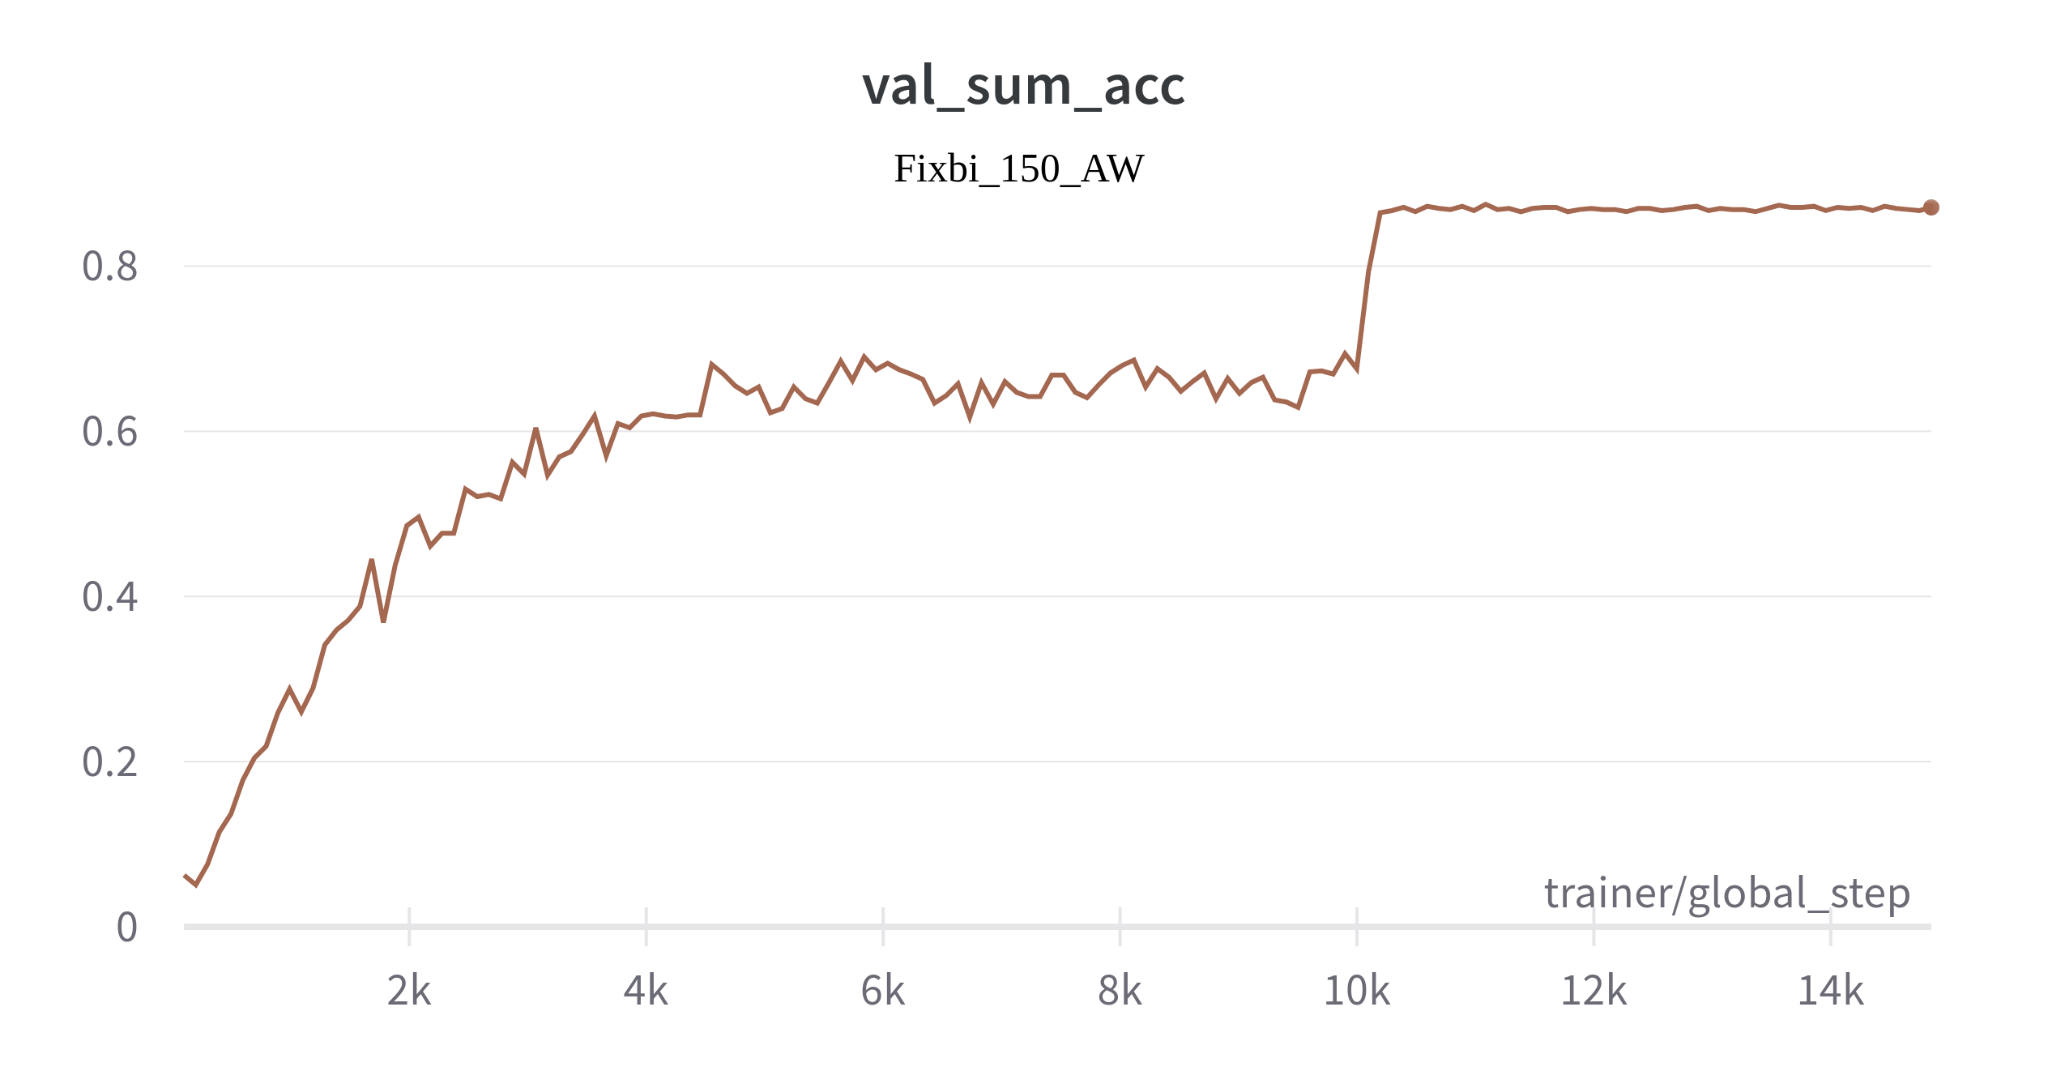
\includegraphics[width=0.8\textwidth]{Figures/Results/fixbi_total.png}
    \caption{The total accuracy of \textbf{Fixbi} model on Amazon and Webcam domains.}
    \label{fig:fixbi_total}
\end{figure}

In the Figure \ref{fig:sdm_tdm}, you can see the separate accuracy of “source-dominant model” (SDM) and “target-dominant model” (TDM) in case of Amazon (source) and Webcam (target) domains.

\begin{figure}[h]
  \centering
  \begin{minipage}[b]{0.49\textwidth}
    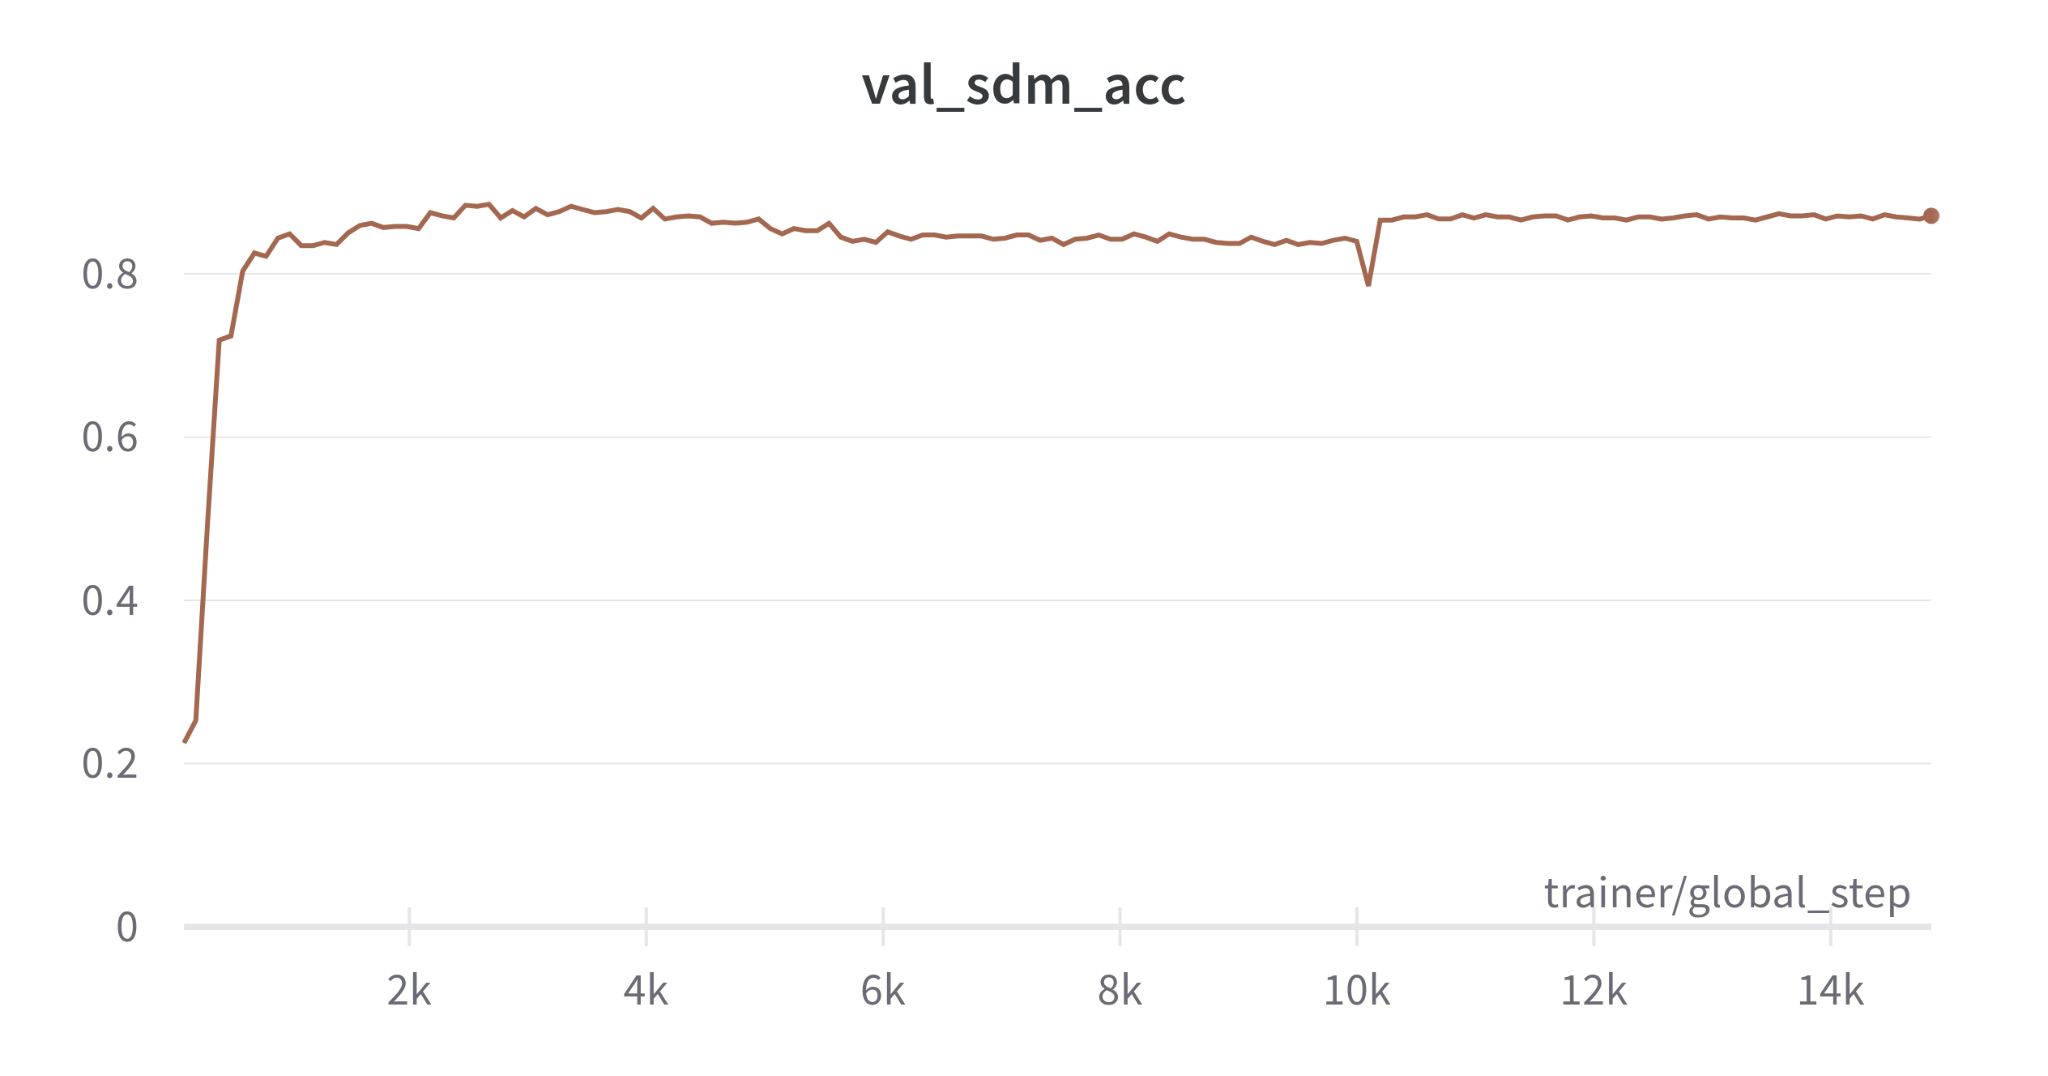
\includegraphics[width=\textwidth]{Figures/Results/fixbi_sdm.png}
  \end{minipage}
  \hfill
  \begin{minipage}[b]{0.49\textwidth}
    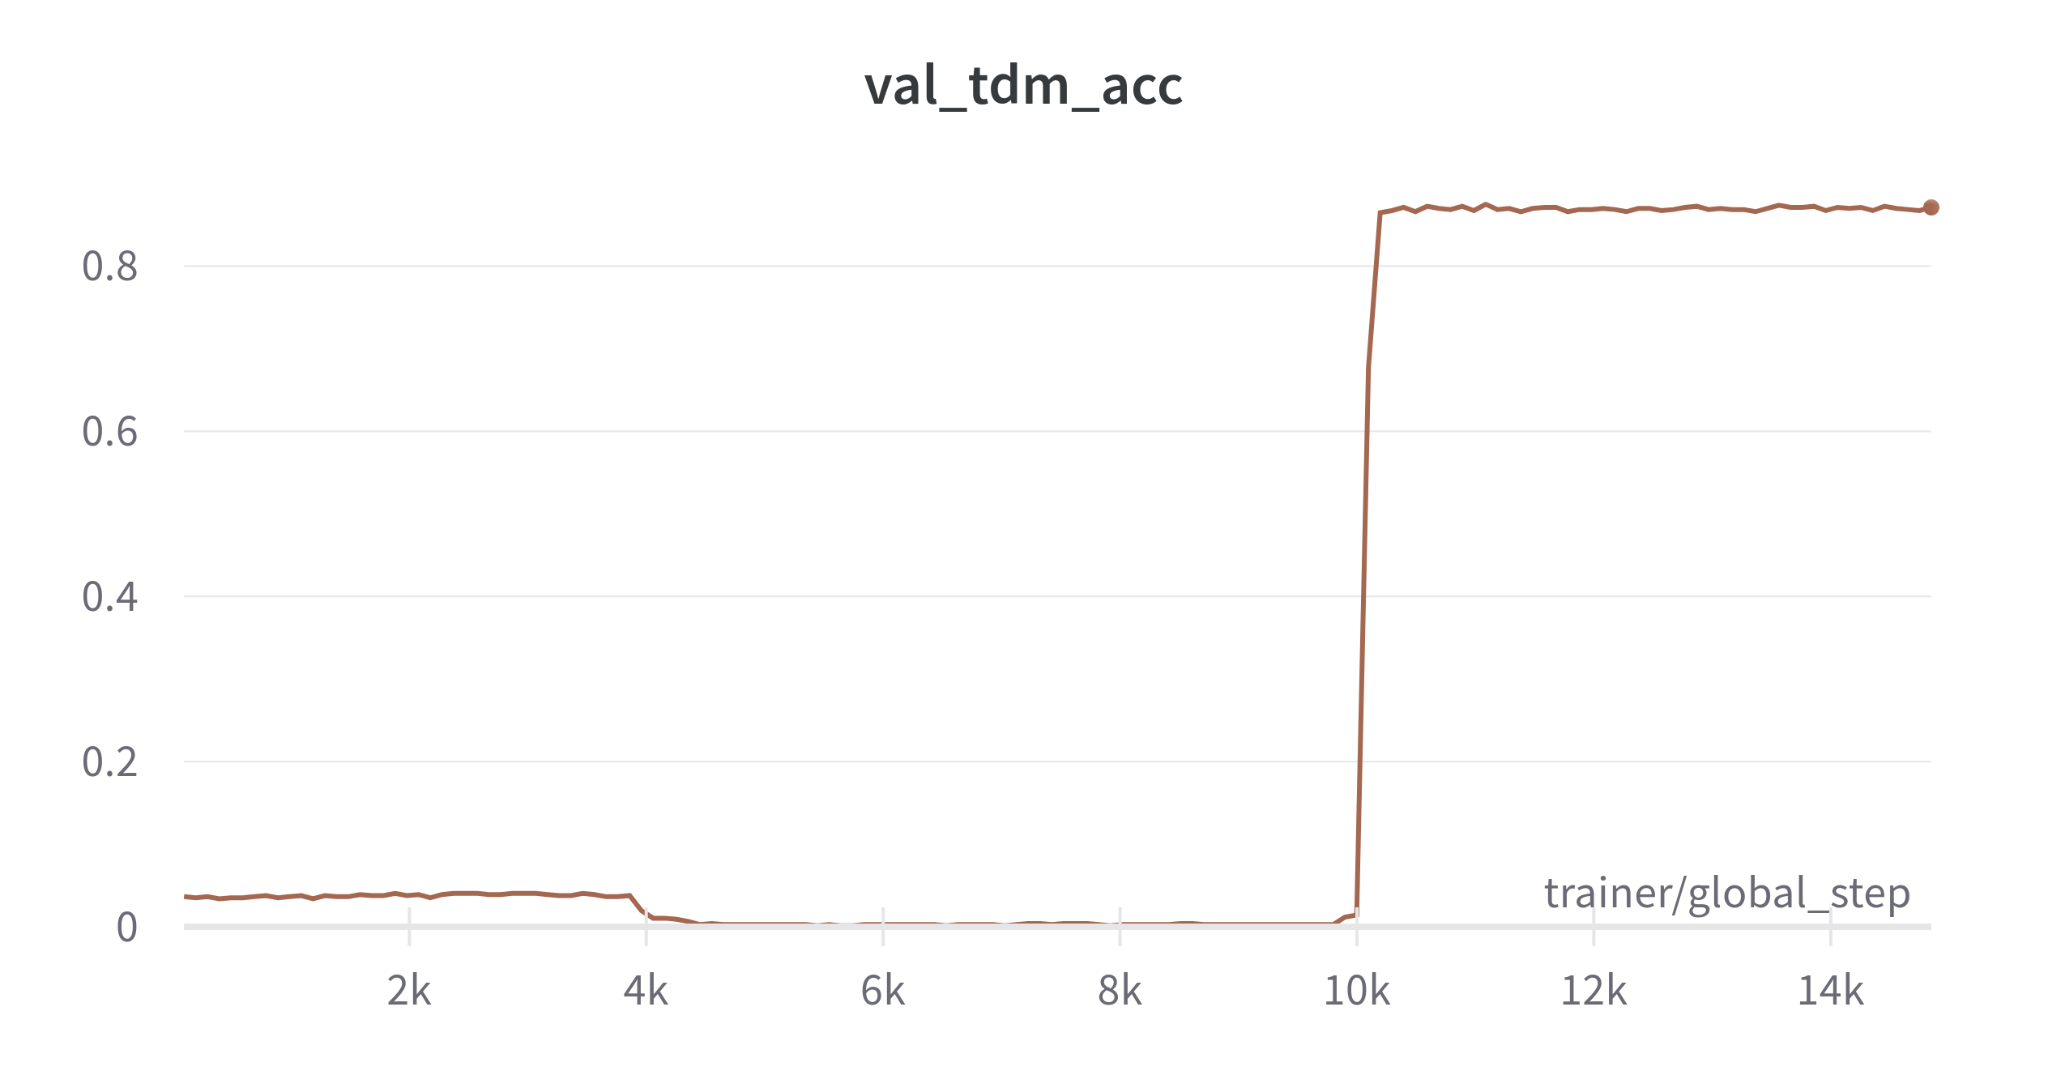
\includegraphics[width=\textwidth]{Figures/Results/fixbi_tdm.png}
  \end{minipage}
  \caption{The separate accuracy of \textbf{Fixbi} “source-dominant model” (SDM) on the left side and “target-dominant model” (TDM) on the right side.}
  \label{fig:sdm_tdm}
\end{figure}

The results for each two domains of Office-31 dataset for \textbf{Fixbi} method are shown in Table \ref{tab:fixbi}.\\
\begin{table}[h]
\centering
\caption{Accuracy on Office-31 for the \textbf{Fixbi} method.}
\label{tab:fixbi}
\begin{tabular}{|r|r|r|r|r|r|r|}
\hline
\multicolumn{1}{|l|}{Fixbi} & \multicolumn{1}{l|}{A$\rightarrow$D} & \multicolumn{1}{l|}{A$\rightarrow$W} & \multicolumn{1}{l|}{D$\rightarrow$W} & \multicolumn{1}{l|}{D$\rightarrow$A} & \multicolumn{1}{l|}{W$\rightarrow$D} & \multicolumn{1}{l|}{W$\rightarrow$A} \\ \hline
1 & 76.88 & 87.11 & 94.66 & 23.19 & 94.38 & 30.15 \\ \hline
2 & 70.1 & 86.72 & 90.89 & 15.23 & 94.38 & 26.03 \\ \hline
3 & 77.08 & 81.77 & 88.54 & 16.01 & 92.92 & 20.63 \\ \hline
4 & 73.96 & 81.38 & 92.78 & 17.8 & 92.88 & 23.45 \\ \hline
\multicolumn{1}{|l|}{\textbf{average}} & \textbf{74.51} & \textbf{84.25} & \textbf{91.72} & \textbf{18.06} & \textbf{93.64} & \textbf{25.07} \\ \hline
\end{tabular}
\end{table}

The \textbf{Fixbi} method was selected for modification, wherein the ratios for SDM and TDM were adjusted, and a domain classifier was added for mixup images. This modified method is named \textbf{DannFixbi}. $\lambda_{sd}$ and $\lambda_{td}$ are set as $0.9$ and $0.7$, respectively. As it was mentioned before, it is used one of the two approaches described in "Contribution" section with domain classifiers for mixup images or separately for each domain. The Table \ref{tab:dann_fixbi} indicates that certain domains exhibit an increase in accuracy as a result of these changes.


\begin{table}[h]
\centering
\caption{Accuracy on Office-31 for the \textbf{DannFixbi} method.}
\label{tab:dann_fixbi}
\begin{tabular}{|r|r|r|r|r|r|r|}
\hline
\multicolumn{1}{|l|}{DannFixbi} & \multicolumn{1}{l|}{A$\rightarrow$D} & \multicolumn{1}{l|}{A$\rightarrow$W} & \multicolumn{1}{l|}{D$\rightarrow$W} & \multicolumn{1}{l|}{D$\rightarrow$A} & \multicolumn{1}{l|}{W$\rightarrow$D} & \multicolumn{1}{l|}{W$\rightarrow$A} \\ \hline
1 & 86.87 & 85.81 & 97.53 & 65.27 & 99.37 & 63.04 \\ \hline
2 & 86.46 & 86.07 & 97.35 & 64.81 & 98.98 & 63.29 \\ \hline
3 & 87.29 & 86.07 & 97.44 & 63.53 & 99.17 & 62.93 \\ \hline
\multicolumn{1}{|l|}{\textbf{average}} & \textbf{86.87} & \textbf{85.98} & \textbf{97.44} & \textbf{64.54} & \textbf{99.17} & \textbf{63.09} \\ \hline
\end{tabular}
\end{table}

Table \ref{tab:all} presents all the obtained results. The \textbf{DannFixbi} method yields the highest accuracy for the A$\rightarrow$D, A$\rightarrow$W, D$\rightarrow$A and D$\rightarrow$W tasks, while the \textbf{Dann} method achieves the best results for the W$\rightarrow$D, and W$\rightarrow$A tasks.

\begin{table}[H]
\centering
\caption{Accuracy on Office-31 for all methods.}
\label{tab:all}
\begin{tabular}{|r|r|r|r|r|r|r|}
\hline
\multicolumn{1}{|l|}{} & \multicolumn{1}{l|}{A$\rightarrow$D} & \multicolumn{1}{l|}{A$\rightarrow$W} & \multicolumn{1}{l|}{D$\rightarrow$W} & \multicolumn{1}{l|}{D$\rightarrow$A} & \multicolumn{1}{l|}{W$\rightarrow$D} & \multicolumn{1}{l|}{W$\rightarrow$A} \\ \hline
\textbf{Source} & 81.04 & 76.17 & 95.79 & 59.93 & 99.44 & 64.25 \\ \hline
\textbf{Dann} & 82.92 & 78.74 & 96.05 & 64.05 & \textbf{99.93} & \textbf{65.01} \\ \hline
\textbf{Mstn} & 77.09 & 72.14 & 91,76 & 33.19 & 99.79 & 49.43 \\ \hline
\textbf{Fixbi} & 74.51 & 84.25 & 91.72 & 18.06 & 93.64 & 25.07 \\ \hline
\textbf{DannFixbi} & \textbf{86.87} & \textbf{85.98} & \textbf{97.44} & \textbf{64.54} & 99.17 & 63.09 \\ \hline
\end{tabular}
\end{table}

Additionally, it is worth noting that an overall assessment of the  methods across all domains can be obtained by calculating the average accuracy (see Table \ref{tab:avg}).

\begin{table}[H]
\centering
\caption{Average accuracy across all domains}
\label{tab:avg}
\begin{tabular}{|r|r|}
\hline
                          & \multicolumn{1}{c|}{Avg} \\ \hline
\textbf{Source}           & 79.44                    \\ \hline
\textbf{Dann}             & 81.12                    \\ \hline
\textbf{Mstn} & 70.57                    \\ \hline
\textbf{Fixbi}            & 64.54                    \\ \hline
\textbf{DannFixbi}        & \textbf{82.85}           \\ \hline
\end{tabular}
\end{table}


To sum up, the new introduced method called \textbf{DannFixbi} outperforms all other methods in visual recognition. The \autoref{section: appendix A}  provides additional results for each domain, allowing for comparisons using the Wilcoxon signed-rank test to determine the statistical significance of the findings (see Tables \ref{tab:AD} -- \ref{tab:WA_wil}). The new method demonstrates statistically significant results in three tasks: A$\rightarrow$D, A$\rightarrow$W, and D$\rightarrow$W, while outperforming all other methods on average (Tables \ref{tab:all_avg} -- \ref{tab:tot_avg}).

\newpage
\section{Conclusion}

In this thesis, the focus was on exploring and implementing methods related to unsupervised domain adaptation. The Office-31 dataset was utilized for evaluating these methods and conducting a comprehensive comparison. The results obtained from the experiments were analyzed, leading to the development of the new \textbf{DannFixbi} method that demonstrated the best performance compared to all the other methods presented. \\

The Office-31 dataset provided a suitable benchmark for evaluating the effectiveness of various unsupervised domain adaptation techniques. By conducting experiments on this dataset, the performance of different methods could be objectively assessed and compared. The analysis of the results shows the strengths and weaknesses of each method, allowing a deeper understanding of their capabilities. \\

Based on the comparative analysis, it was observed that the newly developed method showcased the best results among all the presented methods. The success of the new method can be attributed to its ability to leverage the strengths of existing techniques. By combining the back propagation method with domain classifiers and applying the Fixbi approach, it is possible to identify common features in different domains and share knowledge and insights between networks. This collaborative approach to learning has led to higher performance and increased the overall effectiveness of the method.\\

Overall, this thesis contributes to the field of unsupervised domain adaptation by providing an analysis of existing methods, introducing a new approach, and demonstrating the potential for improving visual recognition tasks across different domains. The results of this study open up opportunities for further study and development of advanced methods in the field of domain adaptation.
